% !TeX encoding = UTF-8
% !TeX spellcheck = en_US
% !TeX TXS-program:bibliography = biber -l zh__pinyin --output-safechars %
% !TeX TS-program = xelatex

\documentclass[a4paper,10pt]{article}

\newcommand{\hwNumber}{3}

% to be `\input` in subfolders,
% ... therefore the path should be relative to subfolders.

\usepackage[UTF8
	,heading=false
	,scheme=plain % English Document
]{ctex}
\usepackage{indentfirst}

\input{../.modules/basics/macros.tex}
\input{../.modules/preamble_base.tex}
\input{../.modules/preamble_notes.tex}

\newcommand{\legacyReference}{{
	\clearpage\par
	\quad\clearpage
	\renewcommand{\midquote}{\textbf{PAST WORK, AS TEMPLATE}}
	\newparagraph
}}

% Settings
\counterwithout{equation}{section}
\mathtoolsset{showonlyrefs=false}
%\DeclareTextFontCommand{\textbf}{\sffamily}
\renewcommand{\midquote}{\quad}
\resizegathersetup{equations=false}

% Spacing
\geometry{footnotesep=2\baselineskip} % pre footnote split
\setlength{\parskip}{.5\baselineskip}
\renewcommand{\baselinestretch}{1.15}

%Title
	\posttitle{
		\hfill\Large\ccbyncsajp
		\par\end{flushleft}%
		\vspace*{-.7ex}\hrule%
	}
	\preauthor{\vspace{-1.5ex}%
		\flushleft\itshape%
	}
	\postauthor{\hfill}
	\predate{\noindent\ttfamily Compiled @ }
	\postdate{\vspace{.5ex}}

	\title{Finite Temperature Field Theory \textnumero\hwNumber}
	\author{\signature Bryan}
	\date{\today}

% List
	\setlist*{
		listparindent=\parindent
		,labelindent=\parindent
		,parsep=\parskip
		,itemsep=1.2\parskip
	}
	\setlist*[enumerate,1]{
		align=left
		,label=\fbox{\textbf{\arabic*}}
		,itemsep=.5\baselineskip
	}

\input{../.modules/basics/biblatex.tex}

%%% ID: sensitive, do NOT publish!
%\InputIfFileExists{../id.tex}{}{}

\begin{document}
\maketitle
\pagestyle{headings}
\pagenumbering{arabic}
\thispagestyle{empty}

\vspace*{-1.5\baselineskip}

\subsection*{QCD Partition Function at $\order{g^2}$}
	\begin{center}
		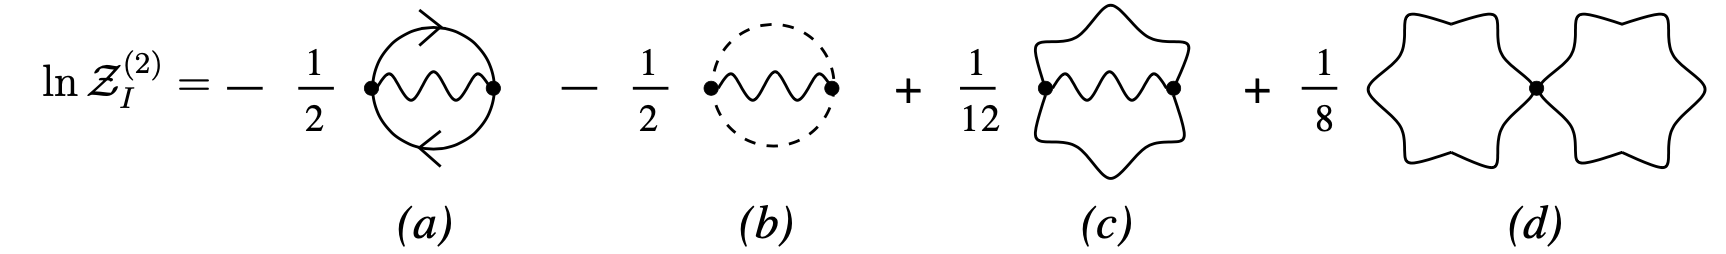
\includegraphics[width=.9\linewidth]{qcd_partition.png}
	\end{center}
	\vspace{-.5\baselineskip}
	\begin{equation}
		\ln \mcal{Z}^{(2)}_I
		= \ln \mcal{Z}^{(a)}
			+ \ln \mcal{Z}^{(b)}
			+ \ln \mcal{Z}^{(c)}
			+ \ln \mcal{Z}^{(d)}
	\end{equation}
	
	The contribution of (a) is given by:
	\begin{equation}
		\ln \mcal{Z}^{(a)}
		= \frac{1}{2!}\,(-1)^1
			\frac{T}{V} \sum_k\,
			\frac{T}{V} \sum_p\,
				\Tr \pqty\Big{
					S(k)\,(g\gamma^\nu T^b)\,
					S(p)\,(g\gamma^\mu T^a)
				}\,
				\pqty{
					\frac{V}{T}
				}\,\delta_{ab}\,
				\Delta_{\mu\nu}(p - k)
	\end{equation}
	Here the trace goes over spinor, color and flavor indices. 
	$S(k)$ is the quark propagator, with suppressed spinor, color and flavor indices, while $\delta_{ab}\,\Delta_{\mu\nu}$ is the gluon propagator, where $a, b$ are adjoint indices; each vertex contributes a $(g\gamma^\mu T^a)$ factor. 
	
	In our convention, $k = (\omega_n, \vb{k})$ stands for the Euclidean 4-momentum with $\omega_n$: the discrete Matsubara frequency. Each $\sum_k$ comes with a factor $\frac{T}{V}$ while each spacetime delta function comes with an inverse factor: $\frac{V}{T}$; this is due to the fact that:
	\begin{equation}
		1 = \int \frac{\dd[4]{k}}{(2\pi)^4}\,
			(2\pi)^4 \delta^4(k - k_0)
		\sim \frac{1}{\beta V} \sum_k
			\beta V \delta_{k,k_0}
	\end{equation}
	Following the same recipe from QED, we can write down:
	\begin{equation}
	\begin{aligned}
		\ln \mcal{Z}^{(a)}
		&= - \pqty\Big{
				\Tr \pqty{
					T^a T^b
				}\,\delta_{ab}
			}\,
			\frac{1}{2}\,g^2
			\frac{V}{T}\cdot
			\frac{T}{V} \sum_k\,
			\frac{T}{V} \sum_p\,
				\Tr \pqty\big{
					S(k)\,\gamma^\nu\,
					S(p)\,\gamma^\mu
				}\,
				\Delta_{\mu\nu}(p - k) \\
		&= - \pqty{
				\frac{N^2_c - 1}{2}\,N_f
			}\,
			\frac{g^2}{288}
			\frac{V}{T} \pqty{
				5T^4
				+ \frac{18}{\pi^2}\, T^2\mu^2
				+ \frac{9}{\pi^4}\, \mu^4
			}
	\end{aligned}
	\end{equation}
	
	The (b) term is structually similar to the (a) term; now the amplitude can be written down simply by replacing the propagator $S(k)\mapsto W(k)$ of the ghost, while the vertex is $(g\gamma^\mu T^a)\mapsto (-igk^\nu T^b)$ instead:
	\begin{equation}
		\ln \mcal{Z}^{(b)}
		= \frac{1}{2!}\,\,(-1)^1
			\frac{T}{V} \sum_k\,
			\frac{T}{V} \sum_p\,
				\Tr \pqty\Big{
					W(k)\,(-igp^\nu T^b)\,
					W(p)\,(-igk^\mu T^a)
				}\,
				\pqty{
					\frac{V}{T}
				}\,\delta_{ab}\,
				\Delta_{\mu\nu}(p - k)
	\end{equation}
	The trace now goes over suppressed \textit{adjoint} indices of $W(k)_{ab} = -\delta_{ab} \Delta(k)$ and $(T_a)_{bc} = f_{abc}$, where $f_{abc}$ is the structure constant of $\mrm{SU}(N_c)$. Therefore\footnote{
		$\Tr \pqty{T^a T^b}_{\mrm{ad}}$ in the adjoint representation is precisely the \textit{Killing form} of the $\mfrak{su}(N_c)$ algebra, which is $2N_c$ times the  $\Tr \pqty{T^a T^b}_0$ in the fundamental representation. 
	}, 
	\begin{equation}
	\begin{aligned}
		\ln \mcal{Z}^{(b)}
		&= - \pqty\Big{
				\Tr \pqty{
					T^a T^b
				}\,\delta_{ab}
			}\,
			\frac{1}{2}\,g^2
			\frac{V}{T}\cdot
			\frac{T}{V} \sum_k\,
			\frac{T}{V} \sum_p\,
				\Delta(k)\,
				\Delta(p)\,
				(-k^\mu p^\nu)\,
				\Delta_{\mu\nu}(p - k) \\
		&= - \pqty{
				\frac{N^2_c - 1}{2}\,2N_c
			}\,
			\frac{1}{2}\,g^2
			\frac{V}{T}\cdot
			\frac{T}{V} \sum_k\,
			\frac{T}{V} \sum_p\,
				\Delta(k)\,
				\Delta(p)\,
				(-k^\mu p^\nu)\,
				(-g_{\mu\nu})\,
				\Delta(p - k)
%		\\
%		&= - \pqty{
%				\frac{N^2_c - 1}{2}\,2N_c
%			}\,
%			\frac{g^2}{288}
%			\frac{V}{T} \,T^4
	\end{aligned}
	\end{equation}
	
%	Now we compute the remaining $\sum_{k,p}$. We have:
%	\begin{equation}
%	\begin{aligned}
%%		& \phantom{{}={}}
%			\Delta(k)\,
%			\Delta(p)\,
%			(k\cdot p)\,
%			\Delta(p - k)
%		&= \frac{1}{k^2 p^2}
%			\frac{k\cdot p}{
%				k^2 + p^2 - 2k\cdot p
%			} \\
%		&= \frac{1}{k^2 p^2}
%			\frac{kp\cos\theta}{
%				k^2 + p^2 - 2kp\cos\theta
%			} \\
%		&= \frac{1}{2k^2 p^2} \pqty{
%			\frac{1}{
%				1 - \frac{2kp}{k^2 + p^2}\cos\theta
%			} - 1
%		}
%	\end{aligned}
%	\end{equation}
%	We first integrate over the $\theta$ angle; note that:
%	\begin{gather}
%		\int_{S^{n+1}} \dd[n+1]{\Omega}
%		= \int_0^\pi \sin^n\!\theta \dd{\theta}
%			\int_{S^n} \dd[n]{\Omega},
%	\\
%		\int_{S^3} \dd[3]{\Omega}
%		= \int_0^\pi \sin^2\!\theta \dd{\theta}
%			\int_{S^2} \dd[2]{\Omega}
%		= \frac{\pi}{2}\cdot 4\pi
%		= 2\pi^2,
%	\\
%		\therefore\quad
%		\int_{S^3} \dd[3]{\Omega}
%			\frac{1}{1 - \alpha\cos\theta}
%		= 4\pi \int_0^\pi \dd{\theta}
%			\frac{\sin^2\!\theta}{1 - \alpha\cos\theta}
%		= 4\pi \cdot \pi\,
%			\frac{1 - \sqrt{1 - \alpha^2}}{\alpha^2},
%	\\
%	\begin{aligned}
%		\int_{S^3} \dd[3]{\Omega} \pqty{
%			\frac{1}{1 - \alpha\cos\theta} - 1
%		}
%		&= 2\pi^2\, \pqty{
%				2\,\frac{1 - \sqrt{1 - \alpha^2}}{\alpha^2}
%				- 1
%			}
%		= 2\pi^2\, \pqty{
%				\frac{1 - \sqrt{1 - \alpha^2}}{\alpha}
%			}^{\!\!2} \\
%		&= 2\pi^2\, \pqty{
%				\frac{k^2 + p^2 - \abs{k^2 - p^2}}{2kp}
%			}^{\!\!2},
%	\end{aligned}
%	\end{gather}
%	
%	\begin{equation}
%	\begin{aligned}
%		& \phantom{{}={}}
%		\int \frac{\dd[4]{k}}{(2\pi)^4}
%		\int \frac{\dd[4]{p}}{(2\pi)^4}\,
%			\Delta(k)\,
%			\Delta(p)\,
%			(k\cdot p)\,
%			\Delta(p - k) \\
%		&= \int_0^\infty \frac{2\pi^2 k^3\dd{k}}{(2\pi)^4}
%			\int_0^\infty \frac{2\pi^2 p^3\dd{p}}{(2\pi)^4}\,
%				\frac{1}{2k^2 p^2}
%				\pqty{
%					\frac{k^2 + p^2 - \abs{k^2 - p^2}}{2kp}
%				}^{\!\!2} \\
%		&\sim \frac{T}{V} \sum_{k^\mu}\,
%			\frac{T}{V} \sum_{p^\nu}\,
%				\frac{1}{2^3 k^4 p^4}\,
%				\pqty{
%					k^2 + p^2 - \abs*{k^2 - p^2}
%				}^2 \\
%		&= 2\cdot \pqty{\frac{T}{V}}^2
%				\sum_{\substack{
%					k^\mu\!,\, p^\nu\\
%					p^2 \le k^2\\[.5ex]
%				}}\,
%				\frac{1}{2^3 k^4 p^4}\,
%				\pqty{2p^2}^2 \\
%		&= \frac{T}{V} \sum_{k^\mu}
%				\frac{1}{k^4}\,
%			\ \frac{T}{V}\!\!\! \sum_{
%					p^\nu\!,\, p^2 \le k^2
%				}\!\! 1\\
%	%%% DEAD END!
%		&= \frac{1}{2^9 \pi^4}
%			\int_0^\infty \dd{k}
%			\int_0^\infty \dd{p}
%				\frac{1}{kp}\,
%				\pqty{
%					k^2 + p^2 - \abs*{k^2 - p^2}
%				}^2 \\
%		&= \frac{2}{2^9 \pi^4}
%			\iint_{k \ge p \ge 0} \dd{k} \dd{p}
%				\frac{1}{kp}\,
%				\pqty{2p^2}^2 \\
%		&= \frac{2^3}{2^9 \pi^4}
%			\iint_{k \ge p \ge 0} \dd{k} \dd{p}
%				\frac{p^3}{k} \\
%		&= \frac{1}{2^6 \pi^4}
%			\int_0^\infty \dd{k}
%			\int_0^k \dd{p}
%				\frac{p^3}{k} \\
%	%%% DEAD END!
%	\end{aligned}
%	\end{equation}
	
	Now we compute the remaining $\sum_{k,p}$. We have:
	\begin{equation}
%		& \phantom{{}={}}
			\Delta(k)\,
			\Delta(p)\,
			(k\cdot p)\,
			\Delta(p - k)
		= \frac{k\cdot p}{k^2 p^2\, (p-k)^2}
	\label{eq:momentum_integrand}
	\end{equation}
	The generic method to carry out such summation is by using the mixed representation of the propagator; for some propagator $D(k)$, we have:
	\begin{equation}
	\begin{aligned}
		D(k) = D(w_n,\vb{k})
		&= \int_0^\beta \dd{\tau}
				e^{-i\omega_n \tau}\,
			T\sum_m e^{i\omega_m \tau}
			D(w_n,\vb{k}) \\
		&= \int_0^\beta \dd{\tau}
				e^{-i\omega_n \tau}\,
			\tilde{D}(\tau,\vb{k}),
	\end{aligned}
	\end{equation}
	\begin{equation}
	\begin{aligned}
		\tilde{D}(\tau,\vb{k})
		&= T\sum_m e^{i\omega_m \tau}
			D(w_n,\vb{k}) \\
		&= T\sum_m e^{i\omega_m \tau}
			\int \frac{\dd{\omega}}{2\pi}
				\frac{\rho(\omega,\vb{k})}{
					\omega + i\omega_0
				} \\
		&= \int \frac{\dd{\omega}}{2\pi}\,
				\rho(\omega,\vb{k})\,
			T\sum_m 
				\frac{e^{i\omega_m \tau}}{
					\omega + i\omega_0
				} \\
		&= \int \frac{\dd{\omega}}{2\pi}\,
				\rho(\omega,\vb{k})\,
			e^{-\omega\tau} \pqty\big{
				1 \pm n_\pm(\omega)
			},
	\end{aligned}
	\end{equation}
	\begin{gather}
		\rho(\omega,\vb{k})
		= \frac{1}{i} \pqty\big{
				D(\omega + i\epsilon)
				- D(\omega - i\epsilon)
			}
		= 2\Im D(\omega + i\epsilon,\vb{k}),\quad
		n_\pm
		= \frac{1}{e^{\beta\omega} \mp 1},
	\end{gather}
	Then the Matsubara sum $\sum_{\omega_n}$ becomes a sum over exponentials like $e^{-i\omega_n \tau}$, which is easier to deal with. However, for this particular problem, there is a shortcut\footnote{
		Reference: Laine \& Vuorinen, \textit{Basics of Thermal Field Theory}. 
	}; notice that the denominator of \eqref{eq:momentum_integrand} is invariant under $p\mapsto k-p$, hence:
	\begin{equation}
	\begin{aligned}
		\sum_p
			\frac{k\cdot p}{k^2 p^2\,(p-k)^2}
		&= \sum_{(k-p)}
			\frac{k\cdot (k-p)}{k^2\,(k-p)^2 p^2} \\
		&= \sum_{p}
			\frac{k\cdot (k-p)}{k^2 p^2\,(p-k)^2} \\
		&= \sum_{p}
			\frac{
				\frac{1}{2} \pqty\big{
					k\cdot p + k\cdot (k-p)
				}
			}{k^2 p^2\,(p-k)^2} \\
%		&= \sum_{p}
%			\frac{k^2}{2k^2 p^2\,(p-k)^2} \\
		&= \sum_{p}
			\frac{1}{2p^2\,(p-k)^2},
	\end{aligned}
	\end{equation}
	\begin{equation}
	\begin{aligned}
		\frac{T}{V} \sum_k\,
		\frac{T}{V} \sum_p\,
			\Delta(k)\,
			\Delta(p)\,
			(k\cdot p)\,
			\Delta(p - k)
		&= \frac{1}{2}\,
			\frac{T}{V} \sum_p \frac{1}{p^2}\,
			\frac{T}{V} \sum_k \frac{1}{(p - k)^2} \\
		&= \frac{1}{2}
			\pqty{\frac{T}{V} \sum_p \frac{1}{p^2}}^{\!\!2}
		= \frac{1}{2}
			\pqty{\frac{T^2}{12}}^{\!\!2},
	\end{aligned}
	\end{equation}
	\begin{equation}
	\begin{aligned}
		\ln \mcal{Z}^{(b)}
		&= - \pqty{
				\frac{N^2_c - 1}{2}\,2N_c
			}\,
			\frac{1}{2}\,g^2
			\frac{V}{T}\cdot
			\frac{1}{2} \pqty{\frac{T^2}{12}}^{\!\!2}
		= - \frac{V}{T}\,N_c \pqty{N^2_c - 1}\,
			\frac{1}{4}\,g^2
			\frac{T^4}{144}
	\end{aligned}
	\end{equation}
	
	
	
	
	
	
	
	
	\legacyReference
	With the metric convention: $
		g\sim\pqty{
			\mathop{-}
			\mathop{+}
			\mathop{+}
			\mathop{+}
	}$, we have:
	\begin{equation}
		\mcal{Z}
		= \int \DD{A^\mu}\,e^{-S}\,
			\delta\bqty\big{
				\pdd{\mu} A^\mu - f
			} \det \bqty{
				\pd^2 \delta^4(x-y)
			}
	\end{equation}
	Here $S$ is the Euclidean action:
	\begin{equation}
		(-S) = \int \dd[4]{x}
			\mcal{L}_{t = -i\tau},\quad
		\int \dd[4]{x}
		= \int_0^\beta \dd{\tau} \int \dd[3]{\vb{x}}
	\end{equation}
	
	For pure QED, we have: 
	\begin{equation}
		\mcal{L}_t
		= -\frac{1}{4}\,F_{\mu\nu} F^{\mu\nu}
	\end{equation}
	Setting $t = i\tau$ is equivalent to carrying out a Wick rotation: $x^0\mapsto -ix^0,\ A^0\mapsto -i A^0$, while:
	\begin{equation}
		g_{\mu\nu} A^\mu A^\nu
		= g'_{\mu\nu} A'^\mu A'^\nu
		\quad\Longrightarrow\quad
		g_{\mu\nu}
		\longmapsto g'_{\mu\nu} = \delta_{\mu\nu}
	\end{equation}
	
	Under this convention, the Euclidean action is formally unchanged; same applies for the gauge-fixing and the ghost term:
	\begin{equation}
		\mcal{L}_{t=-i\tau}
		= -\frac{1}{4}\,F_{\mu\nu} F^{\mu\nu},\quad
		g_{\mu\nu}
		\longmapsto \delta_{\mu\nu},
	\end{equation}
	\vspace*{-1.25\baselineskip}
	\begin{align}
		\delta\bqty\big{
			\pdd{\mu} A^\mu - f
		}
		\quad&\Longrightarrow\quad
		\mcal{L}_{gf}
		= -\frac{1}{2\rho}\,\pqty{
				\pdd{\mu} A^\mu
			}^2,\\
		\det \bqty{
			\pd^2 \delta^4(x-y)
		}
		\quad&\Longrightarrow\quad
		\mcal{L}_{gh}
		\sim (\pd^2\bar{\eta})\,\eta
		\sim -\pdd{\mu}\bar{\eta}\,\pd^\mu\eta,
	\end{align}
	Here we've dropped some total derivative terms in the ghost Lagrangian. The partition function is then reduced to:
	\begin{equation}
		\mcal{Z}
		= \int \DD{A^\mu}\,
			\DD{\bar{\eta}}\,\DD{\eta}\,
			e^{-S'}, \quad
		(-S') = \int \dd[4]{x} \pqty\big{
				\mcal{L}
				+ \mcal{L}_{gf}
				+ \mcal{L}_{gh}
			}_{t=-i\tau}
	\end{equation}
	
	The action can be further simplified by partial integration and dropping boundary terms:
	\begin{equation}
	\begin{aligned}
		(-S') &= \int \dd[4]{x} \pqty{
				-\frac{1}{4}\,F_{\mu\nu} F^{\mu\nu}
				-\frac{1}{2\rho}\,\pqty{
						\pdd{\mu} A^\mu
					}^2
				-\pdd{\mu}\bar{\eta}\,\pd^\mu\eta
			} \\
		&= \int \dd[4]{x} \pqty{
				-\frac{1}{4}\,\pqty{
						\pdd{\mu} A_\nu
						- \pdd{\nu} A_\mu
					} \pqty{
						\pd^\mu A^\nu
						- \pd^\nu A^\mu
					}
				-\frac{1}{2\rho}\,\pqty{
						\pdd{\mu} A^\mu
					}^2
				-\pdd{\mu}\bar{\eta}\,\pd^\mu\eta
			} \\
		&= \int \dd[4]{x} \pqty{
				-\frac{1}{2}\,\pqty{
						\pdd{\mu} A_\nu\,
						\pd^\mu A^\nu
						- \pdd{\nu} A_\mu\,
						\pd^\mu A^\nu
					}
				-\frac{1}{2\rho}\,\pqty{
						\pdd{\mu} A^\mu\,
						\pdd{\nu} A^\nu
					}
				-\pdd{\mu}\bar{\eta}\,\pd^\mu\eta
			} \\
		&\sim \int \dd[4]{x} \pqty{
				-\frac{1}{2}\,\pqty{
						- A_\nu\,
						\pd^2 A^\nu
						+ A_\mu\,
						\pd^\mu \pdd{\nu} A^\nu
					}
				+\frac{1}{2\rho}\,\pqty{
						A^\mu\,
						\pdd{\mu}\pdd{\nu} A^\nu
					}
				+\bar{\eta}\,\pd^2\eta
			} \\
		&= \int \dd[4]{x} \pqty{
				-\frac{1}{2}\,A^\mu\pqty{
						- \delta_{\mu\nu}\pd^2
						+ \pdd{\mu}\pdd{\nu}
						- \tfrac{1}{\rho}\,
							\pdd{\mu}\pdd{\nu}
					} A^\nu
				+\bar{\eta}\,\pd^2\eta
			} \\
		&= -\frac{1}{2}
		\int \dd[4]{x} \pqty{
				A^\mu\pqty{
					- \delta_{\mu\nu}\pd^2
					+ \pqty\big{1 - \tfrac{1}{\rho}}\,
						\pdd{\mu}\pdd{\nu}
				} A^\nu
				- 2\bar{\eta}\,\pd^2\eta
			}
	\end{aligned}
	\end{equation}
	With $\beta = \frac{1}{T}$, expand $A^\mu,\eta$ into dimensionless Fourier modes, and %the above expressions can be reduced to bilinears in momentum space. More specifically, 
	we have:
	\begin{equation}
		A^\mu
		= \frac{1}{\sqrt{TV}}
			\sum_k e^{ik_\nu x^\nu} A^\mu_k,\qquad
		\sum_k e^{ik_\nu x^\nu}
		= V \int \frac{\dd[3]{\vb{k}}}{(2\pi)^3}\,
				e^{i\vb{k}\cdot\vb{x}}
			\sum_{n\in\mbb{Z}} e^{i\omega_n \tau}
	\end{equation}
\pagebreak[3]
	
	\begin{equation}
	\begin{aligned}
		\sum_{p,k}
		\int \dd[4]{x} e^{i\,\pqty{p+k}\cdot x}
		&= \sum_{p,k}
			(2\pi)^4\,\delta^4(p+k) \\
		&= V^2 \int
			\frac{
				\dd[3]{\vb{p}}\dd[3]{\vb{k}}
			}{(2\pi)^6}\,
			\sum_{m,n\in\mbb{Z}}
				\beta\,\delta_{m,-n}\cdot
				(2\pi)^3\,\delta^3(\vb{p}+\vb{k}) \\
		&= \beta V\cdot
			V\int \frac{\dd[3]{\vb{k}}}{(2\pi)^3}\,
			\sum_{n\in\mbb{Z}}
				\int \dd[3]{\vb{p}}
					\delta^3(\vb{p}+\vb{k})
				\sum_{n\in\mbb{Z}}
					\delta_{m,-n} \\
		&= \beta V \sum_k
				\int \dd[3]{\vb{p}}
					\delta^3(\vb{p}+\vb{k})
				\sum_{n\in\mbb{Z}}
					\delta_{m,-n},
	\end{aligned}
	\end{equation}
	\begin{equation}
	\begin{aligned}
		(-S')
		&= -\frac{1}{2TV}
		\sum_{p,k}
		\int \dd[4]{x} e^{i\,\pqty{p+k}\cdot x}
			\pqty{
				A^\mu_p \pqty{
					- \delta_{\mu\nu} (-k^2)
					+ \pqty\big{
						1 - \tfrac{1}{\rho}
					}\,(-k_\mu k_\nu)
				} A^\nu_k
				- 2\bar{\eta}_p\,(-k^2)\eta_k
			} \\
		&= -\frac{\beta V}{2TV} \sum_k
			\pqty{
				A^\mu_{-k} \pqty{
					k^2 \delta_{\mu\nu}
					- \pqty\big{
						1 - \tfrac{1}{\rho}
					}\,k_\mu k_\nu
				} A^\nu_k
				+ 2\bar{\eta}_{-k} k^2\eta_k
			} \\
		&= -\frac{\beta^2}{2} \sum_k
			\pqty{
				A^{\mu\dagger}_{k}
					D^{-1}_{\mu\nu}(k)
					A^\nu_k
				+ 2\bar{\eta}^\dagger_{k} k^2\eta_k
			}
	\end{aligned}
	\label{eq:soft_gauge_fixed_action}
	\end{equation}
	
	Here we've used the reality condition on $A,\eta$, namely $
		A^{\mu\dagger}_{k}
		= A^\mu_{-k}
%		,\ %
%		\bar{\eta}^\dagger_{k}
%		= \eta_{-k}
	$, and defined the $k$--space inverse propagator $D^{-1}_{\mu\nu}(k)$. 
%	We see that $D^{-1}_{\mu\nu}(k)$ is ``diagonal'' w.r.t.\ $k$ but not diagonal w.r.t.\ $\mu,\nu$ indices. However, it is symmetric among the $\mu,\nu$ indices, so it can be diagonalized and compared to the neutral scalar propagator. 
	Similar result applies for $\eta_k$, except that we have to be careful about Grassmann variables. Carry out $
		\int \DD{A^\mu}\,
			\DD{\bar{\eta}}\,\DD{\eta}\,
	$, and we have:
	\begin{equation}
	\begin{aligned}
		\mcal{Z}
		&\sim \pqty\Big{
				\det_{\mu,\nu,k}
				\beta^2 D^{-1}_{\mu\nu}(k)
			}^{-1/2}\,\pqty\Big{
				\det_k
				2\beta^2 k^2
			}^{+1} \\[.5ex]
		&= \prod_k \pqty\Big{
			\beta^{2\times 4\times(-1/2)}
			\cdot \pqty\Big{
				\det_{\mu,\nu}
				D^{-1}_{\mu\nu}(k)
			}^{-1/2}
			\cdot 2\beta^2 k^2
		} \\[-.5ex]
		&= \prod_k \pqty\Big{
			\beta^{-4} \pqty\Big{
				\det_{\mu,\nu}
				D^{-1}_{\mu\nu}(k)
			}^{-1/2}
			\cdot 2\beta^2 k^2
		}
	\end{aligned}
	\end{equation}
	The determinant is evaluated as follows\footnote{
		Reference: \wikiref{https://en.wikipedia.org/wiki/Determinant\#Sylvester's\_determinant\_theorem}{Determinant \texttt{\#} Sylvester's determinant theorem}. 
	}:
	\begin{align}
		\det_{\mu,\nu} D^{-1}_{\mu\nu}
		&= \det_{\mu,\nu} \pqty{
			k^2 \delta_{\mu\nu}
			- \pqty\big{
				1 - \tfrac{1}{\rho}
			}\,k_\mu k_\nu
		} \notag\\
		&= k^8 \det_{\mu,\nu} \pqty{
			\delta_{\mu\nu}
			- \pqty\big{
				1 - \tfrac{1}{\rho}
			}\,\tfrac{k_\mu k_\nu}{k^2}
		} \notag\\
		&= k^8 \pqty{
			1
			- \pqty\big{
				1 - \tfrac{1}{\rho}
			}\,\tfrac{k^2}{k^2}
		} \notag\\[.5ex]
		&= \tfrac{1}{\rho} k^8, \\[1.5ex]
		\mcal{Z}
		&\sim \prod_k 
			\tfrac{2}{\rho}
				\beta^{-4} k^{-4}
				\cdot \beta^{2} k^{2}
		\sim \prod_k \beta^{-2} k^{-2},
		\label{eq:partition_func}\\
		\ln \mcal{Z}
		&\sim - \sum_k \ln \pqty{\beta^2 k^2}
	\end{align}
	
	We see that $\ln\mcal{Z}$ is simply twice the result of a neutral scalar field, with mass $m\to 0$, i.e.\ %
	\begin{gather}
		\ln \mcal{Z}
		\sim -2\times \frac{1}{2}
			\sum_k \ln \pqty{\beta^2 k^2}
		\sim -2\sum_{\vb{k}} \pqty{
			\frac{1}{2}\,\beta E_k
			+ \ln \pqty{
				1 - e^{-\beta E_k}
			}
		}, \\
		\mcal{Z}
		\sim \prod_{\vb{k}} \Bqty{
			\exp\pqty{
				- \frac{1}{2}\,\beta E_k
				- \ln \pqty{
					1 - e^{-\beta E_k}
				}
			}
		}^{2}, \\[1ex]
		\Omega
		= -T\ln \mcal{Z}
		= 2\sum_{\vb{k}} \pqty{
				\frac{1}{2}\,E_k
				+ T\ln \pqty{
					1 - e^{-E_k/T}
				}
			}, \\[1ex]
		p = -\frac{\Omega}{V}
		= -2 \int \frac{\dd[3]{\vb{k}}}{(2\pi)^3}\,
			\pqty{
				\frac{1}{2}\,E_k
				+ T\ln \pqty{
					1 - e^{-E_k/T}
				}
			},
	\end{gather}
	Here $E_k = \norm{\vb{k}}$. Ignore the vacuum contribution to $p$, and we have:
	\begin{equation}
		p = -2T 
		\int \frac{\dd[3]{\vb{k}}}{(2\pi)^3}\,
			\ln \pqty{
				1 - e^{-\norm{\vb{k}}/T}
			}
		= 2\,\frac{\pi^2}{90}\,T^4
	\end{equation}
\subsection*{Summary}
	\begin{enumerate}[label=\arabic*.,itemsep=1ex]
	\item We've completed the calculation of pure QED partition function $\mcal{Z}$ and thermodynamic potential $\Omega$ (energy density $p$) by introducing a ``soft'' gauge fix $\mcal{L}_{gf}$. 
	Alternatively, we can simply impose a ``hard'' Lorenz gauge fix $
		\delta\bqty\big{\pdd{\mu} A^\mu}
	$; this can be achieved by taking $\rho\to\infty$ in the Gaussian packet $
		-\frac{1}{2\rho}\,\pqty{
			\pdd{\mu} A^\mu
		}^2
	$, or by integrating out $A^0$ directly --- similar to \eqref{eq:soft_gauge_fixed_action}, we have:
	\begin{gather}
	\begin{aligned}
		\mcal{Z}
		&\sim \int \DD{A^\mu}\,
			\DD{\bar{\eta}}\,\DD{\eta}\,
			\delta\bqty\big{
				\pdd{\mu} A^\mu
			} \exp \pqty{
				-\frac{\beta^2}{2} \sum_k
				\pqty{
					A^{\mu\dagger}_{k} \pqty{
						k^2 \delta_{\mu\nu}
						- k_\mu k_\nu
					} A^\nu_k
					+ 2\bar{\eta}^\dagger_{k}
					k^2\eta_k
				}
			} \\
		&\sim \int \DD{A^i}\,
			\DD{\bar{\eta}}\,\DD{\eta}\,
			\exp \pqty{
				-\frac{\beta^2}{2} \sum_k
				\pqty{
					A^{\mu\dagger}_{k} \pqty{
						k^2 \delta_{\mu\nu}
						- k_\mu k_\nu
					} A^\nu_k
					+ 2\bar{\eta}^\dagger_{k}
					k^2\eta_k
				}
			}_{\!\!A^0=A^0[A^i]}
	\end{aligned}\\
		A^0[A^i]
		= -\int \pdd{i} A^i \dd{\tau},\quad
		k_\mu A^\mu_k = 0,
		\label{eq:transverse_cond}
	\end{gather}
	Here we've omitted a non-dynamical Jacobian $
		\det \bqty\big{
			\theta(\tau-\tau')
		} = \det \int^\tau \dd{\tau''}
			\delta(\tau''-\tau')
	$. 
	The ghost integral gives the same contribution, while the $A^i$ integral yields:
	\begin{gather}
		\mcal{Z}_A = \int \DD{A^i}\,
			\exp \pqty{
				-\frac{\beta^2}{2} \sum_k
				\pqty{
					A^{\mu\dagger}_k \pqty{
						k^2 \delta_{\mu\nu}
					} A^\nu_k
				}
			}, \\[.5ex]
	\begin{aligned}
		A^{\mu\dagger}_k \pqty{
			k^2 \delta_{\mu\nu}
		} A^\nu_k
		&= A^{i\dagger}_k \pqty{
				k^2 \delta_{ij}
			} A^j_k
			+ A^{0\dagger}_k \pqty{
				k^2
			} A^0_k
%		\\ &
		= A^{i\dagger}_k \pqty{
				k^2 \delta_{ij}
			} A^j_k
			+ \frac{k^2}{\omega^2}\,
			A^{0\dagger}_k \pqty{
				\omega^2
			} A^0_k \\
		&\smash{
			\overset{\eqref{eq:transverse_cond}}{=}
		} A^{i\dagger}_k \pqty{
				k^2 \delta_{ij}
			} A^j_k
			+ \frac{k^2}{\omega^2}\,
			A^{i\dagger}_k \pqty{
				k_i k_j
			} A^0_k
%		\\ &
		= A^{i\dagger}_k \,k^2\pqty{
				\delta_{ij}
				+ \frac{k_i k_j}{\omega^2}
			} A^j_k \\
		&= A^{i\dagger}_k
			D^{-1}_{ij}(k)
			A^j_k,
	\end{aligned}\\[1.2ex]
	\begin{aligned}
		\mcal{Z}_A
		\sim \pqty\Big{
				\det_{i,j,k}
				\beta^2 D^{-1}_{ij}(k)
			}^{\!-1/2}\!\!\!
		&= \prod_k \beta^{-3} k^{-3}
			\pqty{
				1 + \frac{\vb{k}^2}{\omega^2}
			}^{\!\!-1/2}\!\!\!\!
		= \prod_k \pqty{
				\beta^{-4} k^{-4}
				\cdot \beta\omega
			} \\
		&= \prod_k \beta^{-4} k^{-4}
			\prod_{\vb{k}} \prod_n 2\pi n
		\sim \prod_k \beta^{-4} k^{-4}
	\end{aligned}
	\end{gather}
	
	We see that the result from a ``hard'' Lorenz gauge fixing is the same as before, up to a non-dynamical overall coefficient. 
	
	\item In our previous calculations, we notice that after functional integration, $\rho$ is just a non-dynamical overall coefficient in $\mcal{Z}$, hence it can be safely dropped from the final expression; see eq.~\eqref{eq:partition_func}. Therefore, the result is independent of parameter $\rho$. 
	\end{enumerate}

\printbibliography[%
%	title = {参考文献} %
	,heading = bibintoc
]
\end{document}
